\documentclass[14pt]{extreport}
\usepackage{gost}
\usepackage{hyperref}
\usepackage{makecell}
\usepackage{ragged2e}
\justifying
\setcounter{secnumdepth}{5}


\renewcommand{\thefigure}{\arabic{figure}}
\renewcommand{\thetable}{\arabic{table}}


\begin{document}
\pagestyle{empty} 
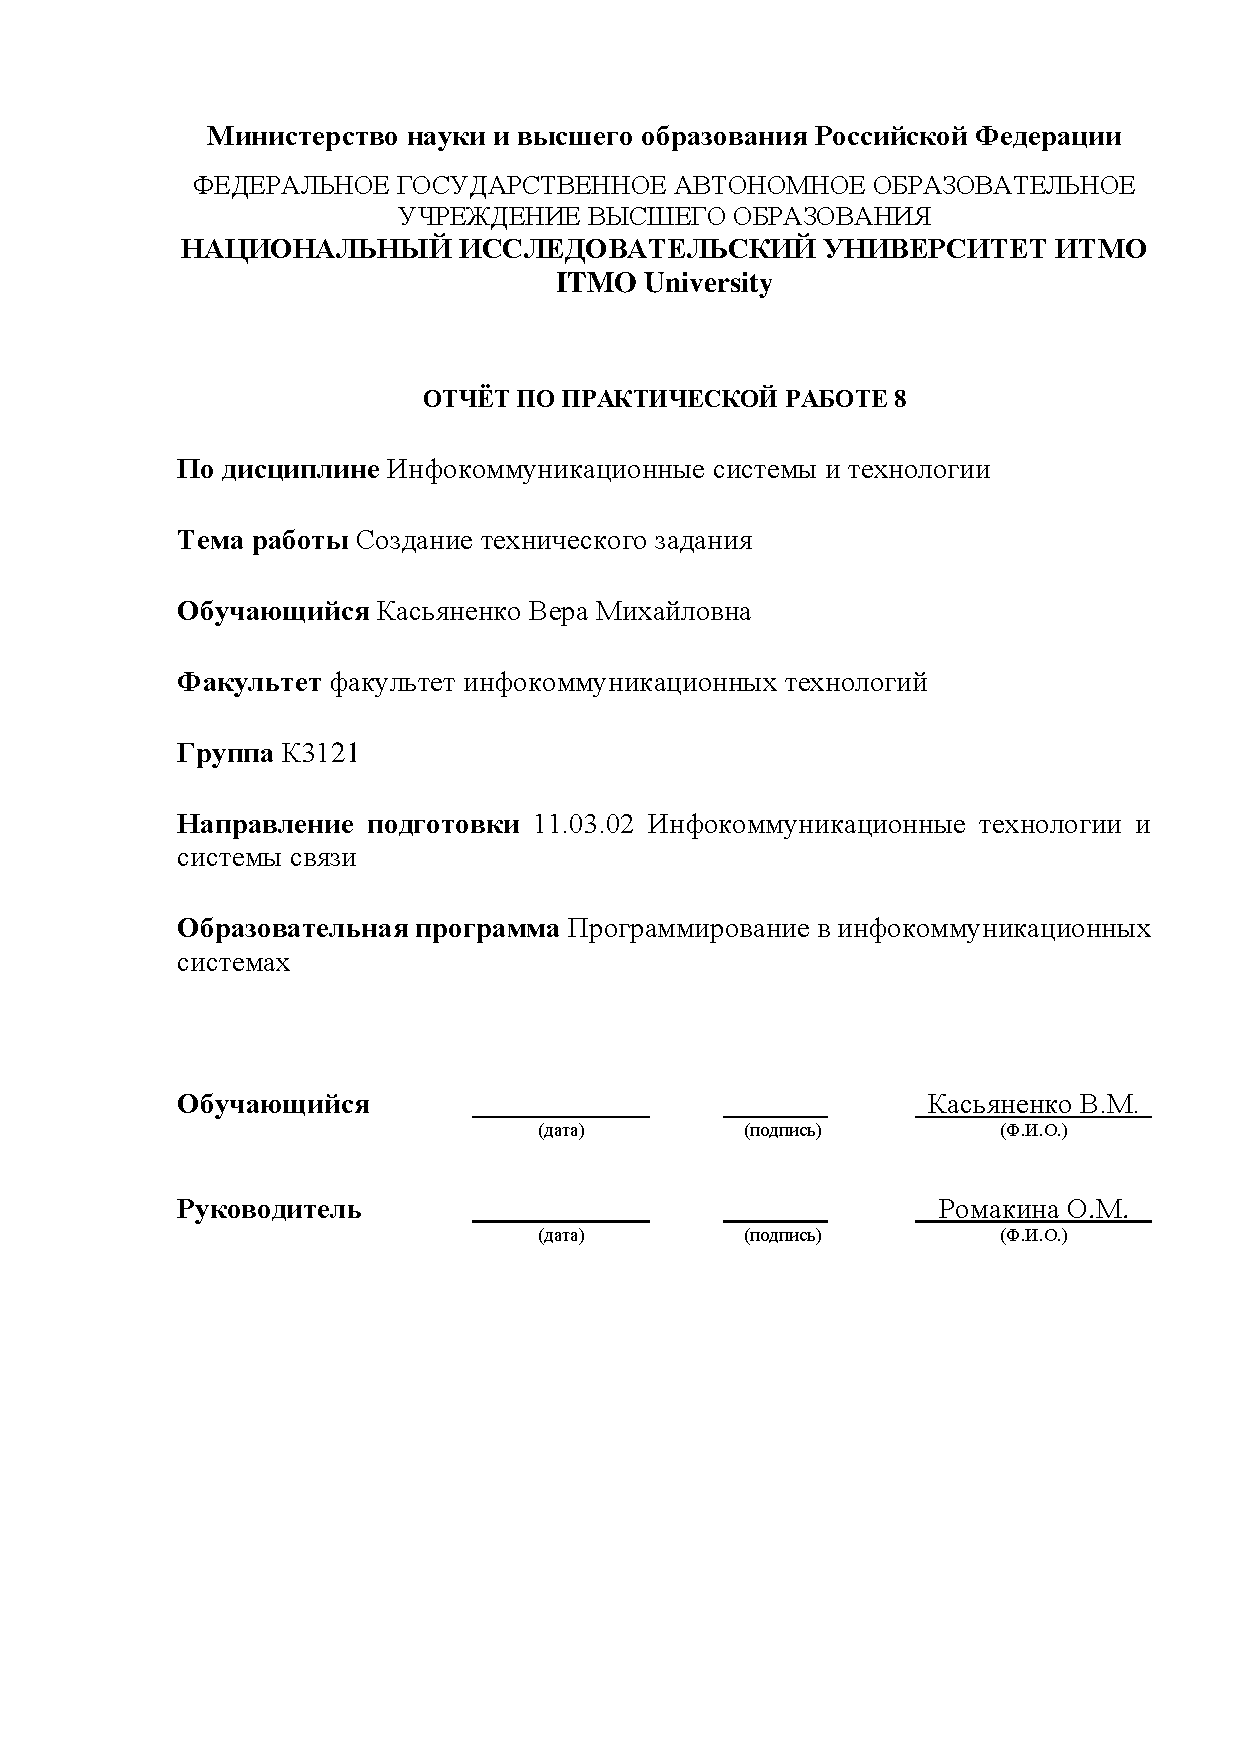
\includepdf[pages=-,pagecommand={}]{titulCourse.pdf}

\pagestyle{plain}
\tableofcontents
 

\intro 

В данном отчете будет составлено техническое задание на создание мобильного приложения OptiTune.

\chapter{Общие сведения}
\section{Наименование системы}
Наименование программного обеспечения: Мобильное приложение OptiTune.

\section{Плановые сроки начала и окончания работы по созданию системы}
30 календарных дней с даты заключения контракта с Заказчиком.

\chapter{Назначение и цели создания системы}
\section{Назначение системы}
Мобильное приложение OptiTune предназначено для использования профессиональными стрелками, охотниками и военными, позволяющее подобрать тюнинг для гладкоствольного и нарезного оружия, улучшая там самым качество стрельбы.

\section{Цели создания системы}

\begin{itemize}
	\item Ускорение поиска необходимого тюнинга для оружия;	
	\item Помощь в нахождении необходимого тюнинга;
	\item Повышение уровня удобства взаимодействия пользователя с интерфейсом системы;
	\item Повышение качества информации.
\end{itemize}


\chapter{Характеристика объектов автоматизации}

Объектом автоматизации является процесс поиска необходимого тюнинга в базе данных запчастей с использованием мобильных устройств.

Под мобильными устройствами в целях настоящего документа понимаются смартфоны и планшетные компьютеры, работающие под управлением мобильных операционных систем (iOS, Android) и имеющие доступ к сети Интернет.

\chapter{Требования к приложению}
\section{требования к системе в целом}
\subsection{Требования к режимам функционирования}
Для системы устанавливаются следующие режимы функционирования:
\begin{itemize}
	\item штатный режим функционирования;
	\item аварийный режим функционирования;
	\item сервисный режим функционирования.
\end{itemize}

Штатный режим является основным режимом функционирования приложения. В этом режиме должна быть обеспечена возможность доступа пользователей 
к приложению.

Система переходит в аварийный режим при возникновении нештатной ситуации и невозможности штатной работы. В случае перехода системы в аварийный режим, обслуживающему персоналу необходимо перевести систему в сервисный режим 
в соответствии с инструкциями, которые должны быть изложены в эксплуатационной документации.

Функционирование приложения при отказах и сбоях серверного оборудования не предусматривается.

В сервисном режиме система должна обеспечивать возможность проведения следующих работ:
\begin{itemize}
	\item техническое обслуживание;
	\item модернизацию аппаратно-программного комплекса;
	\item устранение аварийных ситуаций.
\end{itemize}

\subsection{Требования к численности и квалификации персонала}
Минимальное количество персонала, требуемого для работы программы, должно
составлять не менее 3 штатных единиц — менеджер, модератор и консультант. Весь персонал должен иметь хорошие знания в области оружия и разбираться в нем.

Менеджер должен отвечать за базу данных запчастей запчастей, которую он обязан редактировать в случае обновления или появления новой информации.  В обязанности модератора входит проверка и публикация комментариев пользователей, а консультант должен отвечать на вопросы, которые отправляют ему авторизованные пользователи.

\subsection{Требования к надежности}
Спроектированные архитектурные решения системы должны быть устойчивы по отношению к программно-аппаратным ошибкам, отказам технических и программных средств, с возможностью восстановления ее работоспособности и целостности информационного содержимого при возникновении ошибок и отказов.

Некорректные действия пользователей не должны приводить к возникновению аварийной ситуации.

\subsection{Требования к эргономике и технической эстетике}
\begin{itemize}
	\item Взаимодействие пользователей с приложением должно осуществляться посредством визуального графического интерфейса;
	\item Интерфейс должен быть полностью русифицирован;
	\item Интерфейс не должен быть перегружен графическими элементами и должен обеспечивать быстрое отображение экранных форм;
	\item Пользователь должен иметь возможность указания критериев поиска и выбора информации без привлечения языков программирования;
	\item Элементы интерфейса (кнопки, ссылки) должны иметь названия, позволяющие пользователю однозначно интерпретировать выполняемые 
ими действия.
\end{itemize}

\subsection{Требования к защите информации от \\ несанкционированного доступа}
Система должна обеспечивать защиту авторизованных пользователей от несанкционированного доступа посредством следующих механизмов:
\begin{itemize}
	\item идентификация пользователя;
	\item проверка полномочий пользователя при работе с приложением;
	\item при наборе пароля его символы не показываются на экране, а заменяются одним типом символов.
\end{itemize}

\section{Требования к функциям, выполняемым системой}
Программа должна обеспечивать возможность выполнения перечисленных ниже
функций.

\subsection{Авторизация пользователя}
В приложении должна быть реализована авторизация пользователей. Пользователь может использовать приложение без авторизации, однако он получит доступ к полному функционалу только после завершения регистрации и последующей авторизации.

Процесс регистрации новых пользователей:
\begin{itemize}
	\item при запуске приложения пользователь может пройти регистрацию;
	\item регистрация проводится по логину, который придумает пользователь;
	\item программное обеспечение должно осуществлять поиск и проверку
введенного логина в базе данных пользователей;
	\item после успешной проверки пользователь вводит пароль
\end{itemize}

В случае успешной авторизации зарегистрированный пользователь получает доступ к полному функционалу приложения.

\subsection{Просмотр каталога}
В приложении должна быть реализована функция просмотра всего доступного тюнинга в виде ленты, которую можно пролистывать, а также при нажатии на иконку с какой-либо запчастью должно открываться окно просмотра этой запчасти В этом окне можно посмотреть данную запчасть в виде фотографий и 3D-моделей, которые можно масштабировать, а также рассматривать с разных ракурсов отдельно и на 3D-модели оружия, выбранного пользователем. Это позволит пользователю оценить насколько внешне подходит данная комплектация.

Также в окне просмотра запчасти должна быть доступна к просмотру и сравнению подробная характеристика этой запчасти, в которую входят такие параметры как вес, средняя цена на рынке, высота, ширина, толщина, материал, из которого изготовлена данная запчасть, а также остальные характеристики, доступные для той или иной запчасти. По этим характеристикам должна быть реализована функция сортировки в каталоге, что позволит пользователю быстрее найти необходимую запчасть.

В разделе просмотра каталога также должна быть реализована функция поиска по названию запчасти, в случае, если в базе запчастей не было найдено совпадений, должна выводиться ошибка пользователю. 

Более того, должна быть реализована функция добавления запчасти пользователем в избранное, а также удаление ее оттуда в разделах с каталогом, просмотром отдельных запчастей, а также в специальном разделе, где пользователь может посмотреть все запчасти, которые он добавил в избранное.

Пример дизайна интерфейса представлен на рисунке \ref{int}:
\begin{figure}[H]
\centerline{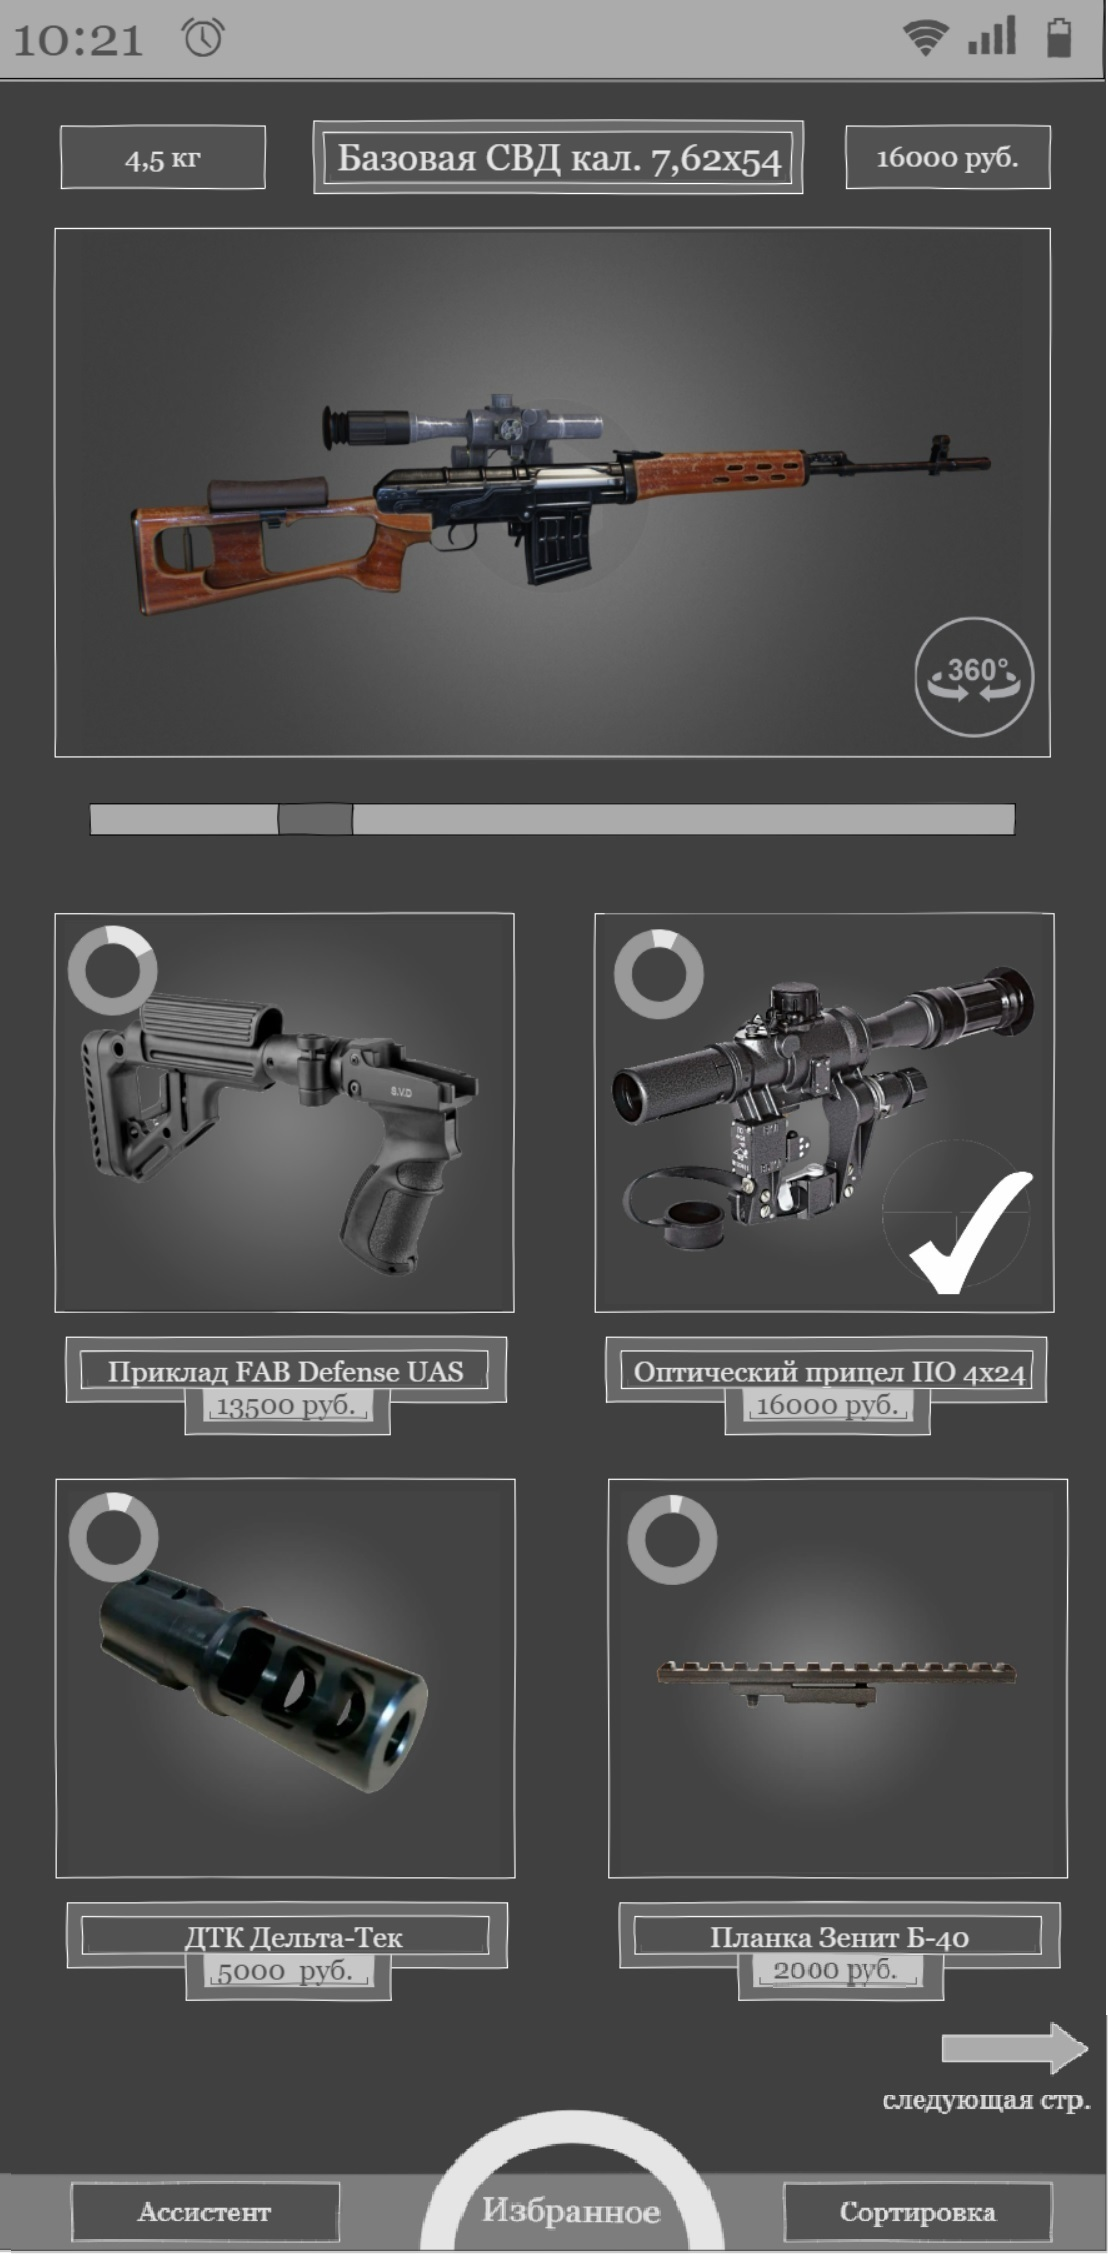
\includegraphics[width=0.52\linewidth]{pic}}
\caption{Пример дизайна интерфейса раздела "Каталог"}
\label{int}
\end{figure}

\subsection{Просмотр и написание комментариев}
В разделе просмотра отдельных запчастей должна быть реализована функция просмотра и написания комментариев с прикреплением приложений в виде фотографий и видеозаписей. Просмотр комментариев должен быть доступен всем пользователям приложения, а функция написания комментариев только авторизованным пользователям.

Процесс публикации комментариев:
\begin{itemize}
	\item написание комментария пользователем;
	\item отправка комментария на проверку модератором;
	\item публикация комментария модератором после успешной проверки. 
\end{itemize}

\subsection{Помощь онлайн-консультанта}
В приложении должна быть реализована функция помощи онлайн-консультанта для авторизованных пользователей. Необходимо обеспечить связь между пользователем и консультантом в отдельном разделе, где пользователь может написать вопрос по интересующей его запчасти или попросить рекомендацию у консультанта, который так же может написать ответное сообщение. 
 
\subsection{Настройки профиля}
Должна быть реализована функция настройки профиля в отдельном разделе, где авторизованный пользователь может изменить свой логин и пароль. Логин так же как и при регистрации проходит проверку на доступность.


\section{Требования к видам обеспечения}

\subsection{Требования к информационному обеспечению}
Проектирование структуры баз данных системы должно осуществляться с использованием инструмента проектирования на основе реляционного подхода.

Система должна быть организована рациональным способом, исключающим избыточную обработку, хранение и передачу информации.

\subsection{Требования к программному обеспечению}
Сервер системы управления базами данных должен функционировать под управлением операционной системы семейства MS Windows или аналогичной операционной системы. В качестве системы управления базами данных  используется Microsoft SQL Server версии 2008 и выше или PostgreSQL версии 9.3.X и выше, либо аналогичная реляционная система управления базами данных, обеспечивающая все функциональные возможности одного из перечисленных продуктов.

На мобильном устройстве пользователя должна быть установлена мобильная операционная система iOS версии 9 и выше или Android версии 4.4 и выше, а также приложение. 

\subsection{Требования к техническому обеспечению}
Техническое обеспечение системы должно максимально и наиболее эффективным образом использовать существующие у Заказчика технические средства.

Должно быть выделено серверное оборудования для сервера баз данных.

\subsection{Требования к организационному обеспечению}
Организационное обеспечение системы должно быть достаточным для эффективного выполнения персоналом возложенных на него обязанностей при осуществлении автоматизированных и связанных с ними неавтоматизированных функций приложения.

К работе с системой должны допускаться сотрудники, имеющие навыки работы за персональным компьютером, ознакомленные с правилами эксплуатации и прошедшие обучение работе с системой.


\chapter{Состав и содержание работ по созданию приложения}
Разработка должна быть проведена в две стадии:
\begin{enumerate}
	\item Разработка приложения:
	\begin{itemize}
		\item проработка структуры приложения;
		\item разработка интерфейса;
		\item добавление запчастей, их характеристик и моделей в базу данных запчастей;
		\item создание функций сортировки и сравнения запчастей по их характеристикам;
		\item разработка системы аутентификации пользователей;
		\item создание функции добавления запчастей в избранное;
		\item создание функции комментирования;
		\item создание функции обращения к онлайн-консультанту;
		\item тестирование, а также устранение выявленных ошибок в работе приложения;
	\end{itemize}
	\item Загрузка приложений в общий доступ:
	\begin{itemize}
		\item загрузка приложения в App Store;
		\item загрузка приложения в Google Play.
	\end{itemize}
\end{enumerate} 


\chapter{Порядок контроля и приемки приложения}
Ответственность за организацию и проведение приемки системы должен нести Заказчик. Приемка системы должна производиться по завершению приемки всех задач системы. При этом необходимо предоставить обеспечение материальной частью (технические средства), проектной документацией и специально выделенным персоналом.

Заказчик должен предъявлять систему ведомственной приемочной комиссии, при этом он обязан обеспечить нормальные условия работы данной комиссии в соответствии с принятой программой приемки.

Завершающим этапом при приемке системы должно быть составление акта приемки.


\chapter{Требования к составу и содержанию работ по подготовке \\
объекта автоматизации к вводу системы в действие}
Для обеспечения готовности объекта к вводу системы в действие провести комплекс мероприятий:
\begin{itemize}
	\item приобрести компоненты технического и программного обеспечения, заключить договора на их лицензионное использование;
	\item завершить работы по установке технических средств;
	\item провести обучение членов административной группы
\end{itemize}


\chapter{Требования к документированию}
Документация должна разрабатываться с учетом требований комплекса государственных стандартов «Информационная технология. Комплекс стандартов на автоматизированные системы»:
\begin{itemize}
	\item ГОСТ 34.601–90 «Автоматизированные системы. Стадии создания»;
	\item ГОСТ 34.003–90 «Автоматизированные системы. Термины и определения»;
	\item ГОСТ 34.602–89 «Техническое задание на создание автоматизированной системы»;
	\item ГОСТ 34.201–89 «Виды, комплектность и обозначение документов при создании автоматизированных систем»;
	\item ГОСТ 34.603–92 «Виды испытаний автоматизированных систем».
\end{itemize}

Документация должна включать следующие документы:
\begin{itemize}
	\item Техническое задание на разработку мобильного приложения;
	\item Программа и методика испытаний приложения;
	\item Руководство менеджера приложения;
	\item Руководство модератора приложения;
	\item Руководство ассистента приложения;
	\item Руководство пользователя приложения.
\end{itemize}

Вся документация должна быть выполнена на русском языке и передана заказчику в печатном виде в одном экземпляре, а также в электронном виде в одном экземпляре в формате doc, docx или pdf.


\chapter{Источники разработки}
Документ, на основе которого разрабатывалось техническое задание и которое должно быть использовано при создании системы:
\begin{itemize}
	\item ГОСТ 34.602-89. Информационная технология. Комплекс стандартов на автоматизированные системы. Техническое задание на создание автоматизированной системы.
\end{itemize}


\conclusions

Был составлен отчет, в котором представлено техническое задание на создание мобильного приложения OptiTune.


\newpage
\begin{thebibliography}{99}

\bibitem{bib1} ГОСТ 34.602-89. Информационная технология. Комплекс стандартов на автоматизированные системы. Техническое задание на создание автоматизированной системы.

\end{thebibliography}

\end{document}